      %http://lattes.cnpq.br/9614728062342745
\documentclass[11pt,onecolumm,a4paper]{article}

% \usepackage[textheight=9.5in,footskip=1pt]{geometry}
\usepackage{geometry}
 \geometry{
 a4paper,
 total={170mm,257mm},
 left=20mm,
 top=15mm,
 }
\usepackage[utf8]{inputenc}
\usepackage[T1]{fontenc}
% \usepackage[pdftex]{graphicx}
 %\usepackage[brazilian]{babel}
% \usepackage[portuguese]{babel}
\usepackage{color}
\usepackage{amsmath}
\usepackage{subcaption}
\usepackage{setspace}
\usepackage[pdftex]{graphicx}
\usepackage[font=footnotesize]{caption}
\usepackage{minted}

\usepackage{float}% If comment this, figure moves to Page 2

\usepackage[extreme]{savetrees} % massa!!!

 % \usepackage[font={small,it}]{caption}
 \usepackage{fancyhdr}
%  \usepackage{physics}
\usepackage{placeins}
% \usepackage{afterpage}
 \usepackage{tabularx}
 
 %\usepackage[dvipsnames]{xcolor}
 \usepackage[table,xcdraw]{xcolor}
 \usepackage{multicol}
 \usepackage{multirow}
 \usepackage{array}
 
\usepackage[
backend=bibtex,
style=nature,
fontsize=10pt,
sorting=none
]{biblatex}
\addbibresource{references.bib}


% ###########
\newcommand{\ket}[1]{\left\vert #1 \right\rangle}
\newcommand{\bra}[1]{\left\langle #1 \right\vert}
\newcommand{\braket}[2]{\left\langle #1 \right\vert\left. #2 \right\rangle}
\newcommand{\ketbra}[2]{\left\vert #1 \right\rangle\left\langle #2 \right\vert}
\newcommand{\D}[1]{\frac{d}{d#1}}
\newcommand{\mean}[1]{\left\langle #1 \right\rangle}
\newcommand{\h}[1]{\hat{#1}}
\newcommand{\m}[1]{\ensuremath{\left\langle #1 \right\rangle}}
\newcommand{\mm}[1]{\ensuremath{\langle #1 \rangle}}
%\newcommand{\trace}[1]{\text{Tr}(#1)}
\newcommand{\trace}[1]{\text{Tr}\left(#1\right)}
% ###########
%\renewcommand{\abstractname}{Resumo}
\usepackage{hyperref}
\hypersetup{
    colorlinks=true,
    linkcolor=blue,
    filecolor=magenta,      
    urlcolor=cyan,
}




\title{ \LARGE Measurement and simulation of Transmon-type superconducting qubits in a 3D cavity: characterization of device energies and characteristic times $T_1$ and $T_2^*$ \\
\normalsize Partial Report}
\date{\today}

\pagestyle{fancy}
\pagenumbering{gobble}

% \date{\selectlanguage{portuguese}\today}
\date{}
\begin{document}
\maketitle
\noindent
\textbf{Grande Área de conhecimento}: Ciências Exatas e da Terra\\
\textbf{Área de Conhecimento}:Física\\
\textbf{Subárea de Conhecimento}: Física da Matéria Condensada\\
\textbf{Aluno}:Daniel G. Benvenutti RA: 169448\\
\textbf{email aluno}: d169448@dac.unicamp.br\\
\textbf{Orientador}: Francisco Rouxinol\\
\textbf{Email orientador}: rouxinol@unicamp.br\\
\textbf{Telefone orientador}: +55(19)3521-5462\\
\textbf{Instituição}: Instituto de Física Gleb Wataghin, UNICAMP\\
\textbf{Áreas de enquadramento da proposta}: Pesquisa Básica\\
\textbf{Áreas de enquadramento CNPq}: Tecnologias Habilitadoras: Materiais Avançados e Nanotecnologia\\
% \begin{itemize} \setlength\itemsep{0em}
% \item Tecnologias estratégicas: Cibernética
% \item 
% \item Tecnologias de Produção: Comunicações 
% \end{itemize}
\textbf{Palavras chaves}: Eletrodinâmica Quântica, Informação e Computação Quântica, Circuitos Supercondutores\\

\begin{abstract}
In this research internship project we continue the steps from previous internships where the theory and experience simulating quantum systems are applied here through real measurements and characterization of superconducting junction transmon quantum bits by obtaining their  parameters like the resonance frequencies of the qubit and cavity, $\omega_{01}$ ,$\omega_{02}/2$  and  $\omega_C$, the coupling parameters $\chi$ and g as well as the relaxation and dephasing times $T_1$ and $T_2^*$ . These will then be validated through simulations using qutip. The work also includes auxiliary tasks such as improving the code executed for the measurement procedures and helping testing, characterizing and optimizing other experimental instruments.

\end{abstract}
%\part*{Resumo}
\part*{Introduction}
\section{Superconducting qubits}
The kind of device used in our laboratory to produce the approximate quantum two level system that can be used as a qubit are superconducting Josephson junction non-harmonic oscillators. Specifically the transmon. 

They work similarly to a quantum harmonic oscillator. This oscillator, unlike the qubit, has infinitely many discrete levels of energy consecutively separated by the same amount of energy. We can understand this quantum harmonic oscillator as the quantized equivalent of a classical harmonic oscillator like an inductor connected to a capacitor in parallel (figure \ref{fig:LC}, where the energy oscillates back and forth between the charge of the capacitor and the magnetic flux of the inductor and where the quantum effects limit the possible energy configurations to these discrete levels as the modes of a confined wave (figure \ref{fig:QHO}. The wave function in this case is confined to the parabolic potential energy well of the harmonic oscillator.

\begin{figure}[h]
\centering
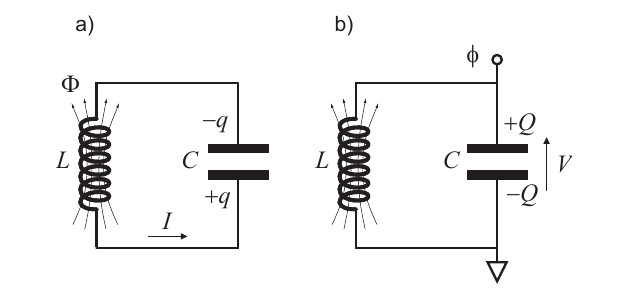
\includegraphics[scale=0.6]{images/9-lc-oscillator.jpg}
\caption{Adapted from: \cite{Girvin2015CircuitQS}. a) State of the oscillator with the energy stored in the inductor`s  magnetic flux and maximum current. b) Energy stored in the capacitor`s charge and maximum voltage. In a mass-spring harmonic oscillator the energy in the capacitor would be analogous to potential energy and (b) would be maximum stretching of the spring, and the energy in the inductor would be analogous to the kinetic energy and (a) would be maximum speed. The voltage would also be the position and the current, the velocity. }
\label{fig:LC}
\end{figure}

\begin{figure}[h]
    \centering
    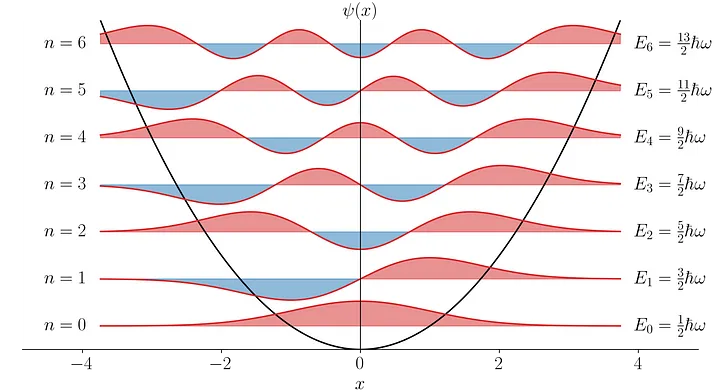
\includegraphics[width=0.5\linewidth]{images/QHO.png}
    \caption{Adapted from \cite{medium_dan_jackson}. Wavefunctions of the energy levels of the quantum harmonic oscillator superposed on the quadratic potential well. We have listed for each energy level it`s energy and it`s quantum number $n$. }
    \label{fig:QHO}
\end{figure}

The difference between this harmonic oscillator and the qubit is that the qubit has a Josephson junction in the place of the inductor. This junction works like an inductor but it has a non-linearity that makes the energy levels of our quantum system not have the same consecutive separation between them. Much like the energy levels of an atom, hence giving the name to this system of an artificial atom. This energy aharmonicity also allows us to excite the first level of the system independently of the other ones. Allowing us to treat this system as two level in certain circumstances. See \cite{Girvin2015CircuitQS}.

The Josephson junction (figure \ref{fig:junction}) is a superconductor wire with a tiny gap made from isolator material separating the two regions of this superconductor. The supercurrent of the cooper pairs of electrons being able to tunnel through this gap creates the behavior of this non-linear inductor mentioned earlier  \cite{gross2016applied}.

\begin{figure}
\centering
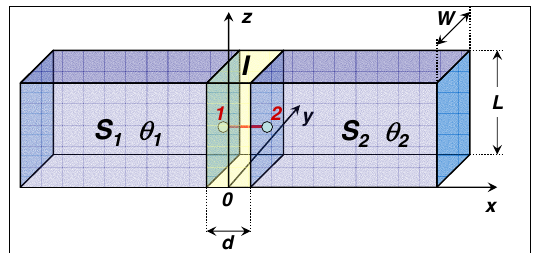
\includegraphics[scale=2.3]{images/superconductor-junction.png}
\caption{Adapted from: \cite{gross2016applied}. Schematics of a Josephson junction. The blue blocks are superconductors separated by a gap with an insulator. The junction is driven by a current and each block will have a distinct phase in the wave function of the cooper pair. The difference in phase between the two blocks has a direct relationship to the current going through the junction. And the rate of change of this phase is determined by the voltage in the junction.}
\label{fig:junction}
\end{figure}


To drive our qubit we can directly apply a signal to the system where we can drive oscillations between the quantum levels when the frequency is close to the frequency of the qubit, much like a light-matter interaction where the atoms are understood as a two-level system. This frequency is defined by the energy of the first level transition. To measure our system we couple the qubit with a metal cavity which works like the quantum harmonic oscillator when alone (bare cavity) and confines an electromagnetic field on it, having a defined transition frequency/energy between it`s discrete energy states. When coupled with the qubit this whole system can be understood with the Jaynes Cumming Hamiltonian approximation that in the proper regime (the dressed cavity) will show how changing the state of the qubit from ground to excited will change also the harmonic transition  frequency of the cavity. Thus by probing the cavity at it`s transition frequency where it will change the magnitude of the signal coming out of it, we can infer the measured state of the qubit by checking if the probe signal output corresponds or not to a signal coming out of a cavity at it`s transition frequency \cite{Naghiloo2019IntroductionQubits}. 

The theory of superconducting qubits with Josephson Junctions is explored in greater depth in the final report of the previous internship made in this laboratory and is available on \hyperlink{https://github.com/Danielgb23/ic-superconductor-qubit}{this github repository}.


These qubits are interesting for applications such as quantum computing as much as their quality parameters are at good enough values. Which would ensure they remain working as quantum two level systems for long enough so that we can do all the intended operations such as several quantum logic gates. This loss of the quantum mechanical aspect of our system is due to effects such as decoherence and other forms of external interference. The main parameters used to determine the quality of our samples are the relaxation time ($T_1$) that is the time constant of the natural exponential decay of the system from the excited state to the ground state and the dephasing time ($T_2$) which measures the exponential time constant loss of the phase property of the qubit making it settle from a superposition into a defined state. 



\section{The goal of the project}
In this internship the goal is to realize measurements on one or several samples of superconducting qubits understanding at the same time the necessary procedures and technical steps to actually do the measurement and also the physics behind how the quantum mechanical system works, having thus a full understanding of the process in theory and practice. The end goal of these measurements is the characterization of the quality parameters of these samples like the Relaxation ($T_1$) and dephasing ($T_2$) times.

To validate this understanding the intern will also do simulations of the real system to validate the theory learned in previous internships with the experimental data. As well as compare the experimental values with the values expected from characteristics of the samples defined by the fabrication parameters.

The intern will also use his experience with python programming for data analysis gained in other internships to improve the execution of the measurement procedures and simulations used in the laboratory.

\part*{Methodology and activities}
\section{The measurement procedures}
The equipment setup and procedures used to measure the superconducting transmon qubits's quantum properties are similar to the used in  \cite{Naghiloo2019IntroductionQubits}. 
\subsection{The VNA setup}
In this setup we use a VNA (Vector Network Analyzer)  which will scan the cavity`s input with several frequencies and collect the phase and amplitude of the output of said cavity. To excite the qubit we connect the drive wire terminal directly to an RF source controlled by our computer.

\subsection{Finding the cavity}
The first step of measuring a sample is finding out the frequency of excitation of the cavity. We can observe the spectrum around the expected value for this frequency looking for a valley where there's absorption of the signal by the cavity and also checking if we can see the characteristic transition of phase given by the cavity's absorption at this valley to be sure it really is the frequency we are looking for. The next step to ensure we are at the cavity's transition is the punchout procedure.

\subsection{The punchout}
With the punchout we scan again the frequency of the cavity around the value of the transition with the VNA. But this time we vary the amplitude of our input signal by using a variable attenuator mounted before the input of the cavity. In a low intensity signal setting the cavity is in the dressed state and has a certain frequency of transition because it interacts with the qubit. But if we increase the intensity after a certain amount we overwhelm the qubit with photons inducing a current on it much above the critical current of the junction, in practice changing the cavity to the bare state (not coupled to the qubit) and thus changing it's transition frequency. 
So if there's really a working qubit  on our sample we observe distinct transition frequency for the cavity in high and low power \cite{Naghiloo2019IntroductionQubits}.
\subsection{The Two Tone Spectroscopy}
Now that we know the cavity's transition frequency and a intensity of the cavity signal where it is at the desired regimen where our approximations apply, which would be at the low attenuation. We can try to find the qubit experimental transition frequency. To do that we continue using the VNA but only collecting data points at the transition of the cavity. Effectively if the transition of the cavity changes because of the state of the qubit went to excited, the cavity stops absorbing the signal at the small frequency range defined at the VNA, at the peak of the cavity transition, and the signal at the output goes up. Therefore if we excite the qubit with a signal and scan the frequency of this signal, we will get a peak at the output of the cavity where the frequency of the qubit signal made it go to the excited state. By setting the scan of the qubit frequency around the expected value infered from the fabrication procedure we can find out the experimental qubit transition frequency.

We can also see half of the frequency of the transition from the ground state to the second energy level of the qubit with a high enough intensity of the qubit signal but with much lower contrast. This happens because there can be a two photon transition between these energy levels. With this transition we can found the aharmonicity of our qubit or how much it deviates from a regular harmonic oscillator.

\subsection{The pulsed setup}
To continue the characterization procedure of the qubit we now switch to the pulsed setup. So instead of using the VNA to measure the cavity response we do pulses generated by a switch (that can generate arbitrary signals with a very fine resolution) and to recover the data we use an Alazar capture board that can collect samples per second on the order of hundreds of MHz. 

The signal sourced to the cavity is treated through the Heterodyne technique so that we can reduce the frequency of the signal of it's output. This way we can capture the phase and amplitude of the signal in our capture board with a low sampling rate while still going up to the excitation frequency in the cavity. We do that by generating a signal on an RF source around the frequency of the cavity ($\approx 7GHz $) and mixing it with a signal of 240MHz. We then input this mixed signal  which has the frequency of the RF source plus the 240MHz on the cavity where it will have it's phase and amplitude changed according to the quantum system's parameters. The output signal of the cavity is then mixed again with the same signal generated from the RF source, though now we filter the difference between the two mixer inputs recovering a signal of 240MHz with the amplitude and phase characteristics imprinted by the cavity. This signal can be captured by the capture board where it will be digitally treated with the Homodyne technique to recover the quadratures I and Q that tell us about the phase and amplitude of our signal.

The signal for the qubit can be generated in several ways. The two used during my internship were generating, in a switch, DC square pulses on the I and Q ports of an IQ mixer that has an IF input generated by an RF source. This way we can control the amplitude and phase of the RF's source signal and shape it in the form of pulses. Though the problem of this technique was that when the I and Q voltages were zero some signal still went through the mixer interfering with the qubit during for example the measurement period. We called this the "leakage". The other possible way was generating the RF signal pulses for the qubit directly from the switch. Though for some reason the stage of the dilution refrigerator where the sample was started heating with this setup.

We then repeat the Punchout and Two Tone procedures with the pulsed setup to verify if everything is proper.

\subsection{The Rabi Oscillation}
With the experimental excitation frequency of the qubit and of the cavity we can start doing Rabi Oscillations. For that we setup a pulse sequence where we do an excitation pulse on the qubit with it's the frequency and a variable duration and then we do a measurement pulse. With the average of several pulse sequences we get an expected value for the state of the qubit for a certain pulse duration. The behavior of this expected value in function of the duration follows a damped cosine, characteristic of the Rabi oscillation of a quantum system.

By fitting the data into an damped cosine or just getting the time duration of the first peak we can get the period of the Rabi Oscillation, and with half of this period we have the $\pi$ pulse duration which is the pulse that excites the qubit from the ground state to the excited state. With a $\pi/2$ pulse or a quarter of the period we change the qubit from the ground state to a state of superposition.

The Rabi Oscillation also depends on the detuning $\Delta$ from the ressonance frequency of the qubit and the amplitude of the drive signal $A$ \cite{Naghiloo2019IntroductionQubits}:
\begin{equation}
    P_e(t)= \frac{A^2}{A^2+\Delta^2} \sin^2(\frac{\sqrt{A^2+\Delta^2}}{2}t)
\end{equation}
 This equation is for an isolated system so it doesn't have the damping unlike the experimental oscillation.
 
\subsection{The $T_1$ measurement}
To do this measurement we use a $\pi$ pulse to excite the qubit and wait a duration after which we measure the qubit state. The expected value of this measurement will be an exponential decay in function of the time duration interval between the excitation and the measurement. The time constant of this decay is our $T_1$ parameter.

\subsection{The $T_2^*$ measurement or Ramsey Interferometry}
To do the Ramsey interferometry, which is the procedure also used in atomic clocks, we do two $/pi/2$ pulses separated by a duration $T$. The expected value of the qubit state will vary according to a damped cosine oscillation in function of this period $T$. The frequency of this oscillation depends on the detuning of the pulses from the qubit's resonance frequency. if the excitation signal is a perfect resonance the oscillation has 0 frequency, thus we have to excite the qubit with a slight detuning to do this measurement. 

From the damped cosine's decay time constant we get our $T_2^*$ parameter which is less or equal to the actual $T_2$.

\subsection{The $T_2^{\textbf{ECHO}}$ measurement }
In this measurement we do like the Ramsey interferometry but with a refocusing $\pi$ pulse right in the middle of the two $pi/2$ pulses with two equal intervals of length $T$ between the pulses. This refocusing pulse changes the direction of precession of the qubit when it's in superposition, canceling out the precession before the $\pi$ pulse with the precession after the $\pi$ pulse. So that we get just an exponential decay on the expected value of the measurement and not an oscillation like we have at the Ramsey interferometry. The double of this decay's time constant is our $T_2^{\textbf{ECHO}}$ because $2T$ is the total time of free evolution/dephasing in our experiment.


\section{Improving the code of the measurement procedure}
\subsubsection{ The original setup} The experiments in the laboratory are executed in python through Jupyter notebooks that use self-made libraries to interact with the measurement equipment through the py-visa API. A single computer is used to control the measurement setup and is linked to the experimental devices through a regular IP addressed network.  The data is recorded into npz files saved directly into this computer. The equipment setup to refrigerate and pump the vacuum in the experiment's chamber is separated from this measurement setup. 

\subsubsection{Modifications} 

The procedure to improve the code begins with applying good coding practices in python for data analysis. Like avoiding using for loops when there's already a function implemented for that in the library used (ex. using numpy's fill method instead of assigning each element in an array) , avoiding repetition and unnecessary code which increases the likelihood of mistakes, makes the code inefficient and hinders modification.

Other modifications included using the plotly library for plotting instead of matplotlib because the plotly graphs are interactive and allow the users to easily get information about their plots like the coordinates of a determinate data point or fit instead of having to manipulate the code to get this information. A trade off is that the plotly library although more powerful is less intuitive to use.

The notebooks for the experimental procedures were also modified to fit a certain standard where the parameters of the experiment are separated from the execution in different code cells. In a way making it encapsulated. Though not entirely to allow the users the flexibility of easily modifying the execution if needed. If the procedures were already reliable enough to become standardized then it would be interesting to encapsulate them under the guidelines of Object Oriented programming with an API to simplify the code that is executed to run a series of measurements.

A data object for the experiment notebook was generated to share parameters across all the different measurements. Like setting up the qubit transition frequency to be set as a parameter in the Rabi and Ramsey measurements for example. This prevents the user from having to modify a parameter on all measurement code cells if needed and saves the user from a greater risk of mistakes from forgetting to change one or other parameter.

The save files now record more metadata from the experiments. An API to recover the temperature of the sample can allow for this data to also be stored for each data point.

\paragraph{Pulse Libraries} In the laboratory's code for controlling the switch I created new types of pulses (inheriting the Pulse class) to be used directly by the switch without a mixer, the 'GaussianCosPulse' and the 'GaussianBorderCosPulse', that have both the envelope and the oscillation to excite the qubits, and are respectively a cos with a gaussian envelope and the other a rectangle envelope with half gaussian curves on the borders. In the way the other pulses were implemented, the curve was generated directly based on an absolute time vector in the 'build' method. I reorganized it to have an 'envelope' method with a relative time vector input (beginning at 0 until the total length of the pulse as a function of t). This method is then called in the 'build' method with an absolute time oscillation. The absolute time for oscillation is necessary to maintain phase coherence between different pulses by given them a common reference for the phase. Separating the envelope part from the oscillation improves code readability and makes it easier to implement modified versions of it with different envelopes based on the current code.

Below is the class declaration of the 'GaussianCosPulse':
\begin{minted}{python}
from measurements.waveforms.Pulse import Pulse
import numpy as np
 
 
class GaussianCosPulse(Pulse):
    """
    This class defines a pulse to be sent to the AWG.
    """
 
    def __init__(
        self, amplitude, sigma, frequency, length=-1, length_factor=7, phase=0
    ):
        """Gaussian enveloped cosine wave
 
        Args:
            amplitude (_type_): vp
            sigma (_type_): gaussian std
            frequency (_type_): cos frequency
            length (_type_,optional): total length in seconds, if set ignores length_factor
            length_factor (_type_,optional): length in number of times the std sigma
            phase (int, optional): cosine phase. Defaults to 0.
        """
        # sigma dependant length
        if length <= 0:
            self.length_factor = length_factor
            super().__init__(length_factor * sigma)
        # length explicitely set by user size independant of sigma internally
        else:
            super().__init__(length)
 
        self.amplitude = amplitude
        self.sigma = sigma
        self.frequency = frequency
        self.phase = phase
 
    def envelope(self, t):
    """
    Time relative envelope of the pulse
    """
        s = (
            self.amplitude
            * np.exp(-(((t + (-self.length) / 2)) ** 2) / self.sigma**2 / 2)
        )
        return s
 
    def build(self, timestep, initial_time=0):
    """
    Builds the combination of the time relative envelope and time absolute oscillation.
    The oscillation must be in absolute to ensure phase coherence between different pulses.
    """
        t = np.arange(initial_time, initial_time + self.length, timestep)
 
        return t, (self.envelope(t - initial_time)
            *np.cos(2 * np.pi *self.frequency * (t) + self.phase)
        )
\end{minted}

\section{The qubit excitation Mixer Characterization}

The mixer is a RF minicircuit that uses a nonlinearity to multiply two signals. I characterized the mixer of the model IQ0307LXP. It multiplies the signal in the LO port with the signal from the I port and it sums this signal to the multiplied signal of the LO port and Q port with a 90º phase. In the time domain we could say we are enveloping the signal in the LO port with the signal in either I or Q and summing them both . In the frequency domain using trigonometric rules we can verify that multiplying two cosines will give us a signal with cosines that have the sum and the subtraction of the two input frequencies (LO and I/Q). That all plus some harmonics and leaks of the original signals.

The signal in the LO port in our case is the main signal with a cosine at the qubit resonance. We then can use pulses (usually square) in I to generate a phase zero pulse of the qubit, one in Q to generate a phase 90º pulse and any amplitude in I and Q combination to generate other phases. Nevertheless we did not use this setup for the excitation of the qubit in my measurements and instead used the switch that at first was only resposible for generating the square pulses because of the leakage of the mixer that was interfering with the qubit state.

\subsection{Leakage}
We can verify in figure \ref{fig:leakage} that the higher the frequency the lower is our leakage. The LO amplitude doesn't make much difference.

\begin{figure}[H]
    \centering
    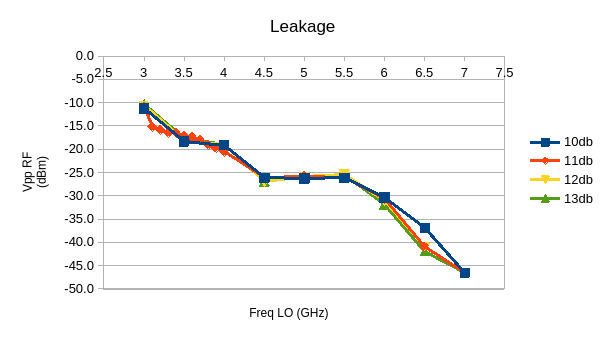
\includegraphics[width=0.5\linewidth]{images/leakage.png}
    \caption{Leakage of the mixer using different LO signals with I and Q with no signal.}
    \label{fig:leakage}
\end{figure}

\subsection{Signal/leakage ratio}
We can diminish the influence of the leakage by attenuating the mixer output and using a high value in the amplitude of I and Q which gives us a greater signal/leakage ratio. Though it's much more convenient to just use the switch directly for the reason that it will not have the leakage problem and it can generate the necessary frequency. We also get better signal to leakage ratios on higher frequencies.

\subsection{I and Q output amplitude difference}
The higher the frequency the higher the difference between the effect the two inputs I and Q have on the output. The user manual for the IQ0307LXP mixer advises to use an attenuator to compensate the difference that might exist on the input with higher output (for example at 7GHz we attenuate I by 3dB with figure \ref{fig:mixer-diff} as reference).
\begin{figure}
    \centering
    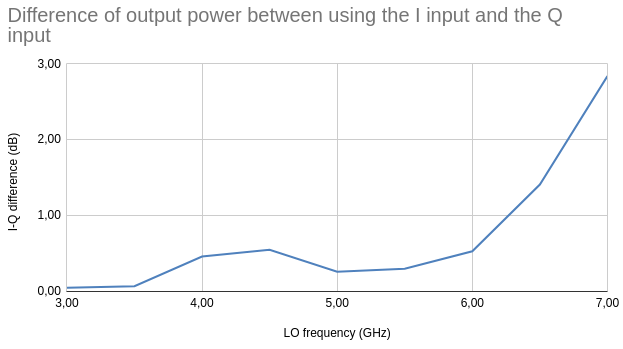
\includegraphics[width=0.5\linewidth]{images/mixer-I-Q-diff.png}
    \caption{Difference in dB of what you get by using either only the I input or the Q input with the maximum AWG amplitude and 11dB in the LO input. The graph displays the ratio (or subtraction in dB) or both values ($P_I-p_Q$)}
    \label{fig:mixer-diff}
\end{figure}


\section{The simulations}
\emph{Scheduled to be finished after the delivery of this first report and therefore to be added into the next.}

\part*{Results}
\section{Measurements}
Given the constraints on time and the availability of the experiment equipment I wasn't able to do a systematic and throughout measurement of all samples. But in the combination you can find most of a qubit's relevant properties.

\subsection{The 2QTII sample}
The expected parameters for this qubit calculated from the project's dimensions and parameters are 7GHz for the cavity resonance and 4.38GHz for the qubit resonance.

\subsubsection{The punchout}
From these measurements we get the value of the cavity resonance at low power (dressed state) of 7.0207GHz that will be used to calibrate the measurement of the qubit. We also have chosen the attenuation of 50dB to be the closest to the regimen that fits best our approximations.
\begin{figure}[H]
    \centering
    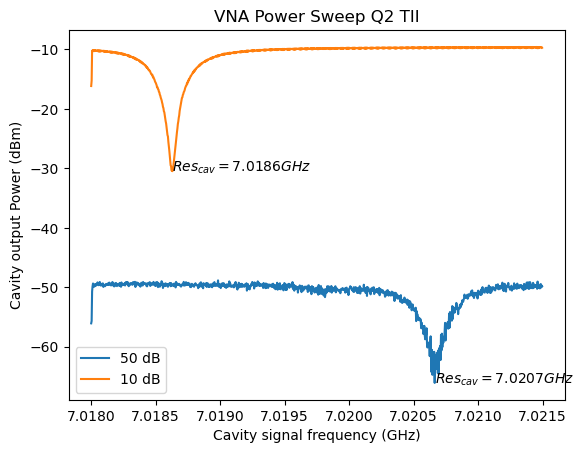
\includegraphics[width=0.5\linewidth]{images/punchoutvna.png}
    \caption{Frequency domain scan of the cavity for two different powers, with 50dB and 10 dB attenuation, and respective resonance frequencies of 7.0207GHz and 7.0186GHz. The 10dB has high power and therefore corresponds to the bare cavity  resonance frequency, the 50dB resonance corresponds to the dressed cavity.}
    \label{fig:TIIQ2-vna-punchout}
\end{figure}

\begin{figure}[H]
    \centering
    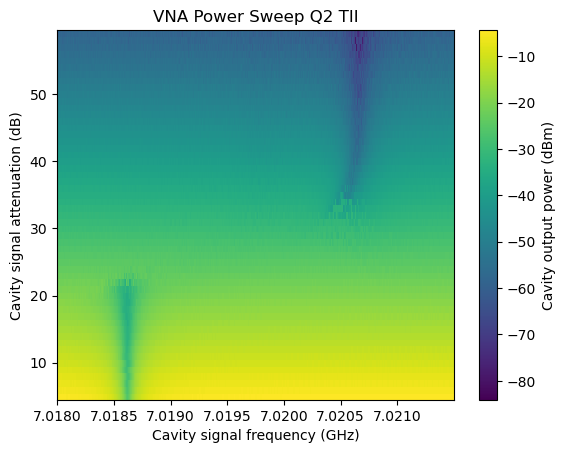
\includegraphics[width=0.5\linewidth]{images/punchoutvnamap.png}
    \caption{Frequency domain and power scan map of the cavity. The two vertical valley lines correspond to the bare and dressed cavity resonances.}
    \label{fig:TIIQ2-vna-punchout-map}
\end{figure}

\subsubsection{The Two Tone Spectroscopy}
We got from this measurement the qubit's resonance frequency for the first transition $\omega_{01}$ of 4.4540GHz and for the two photon transition from the ground to the second level $\omega_{02}/2$ of 4.1460GHz. Giving an aharmonicity to the qubit of $\omega_{01} -\omega_{12}=2\omega_{01} -\omega_{02}=$ 616MHz.
\begin{figure}[H]
    \centering
    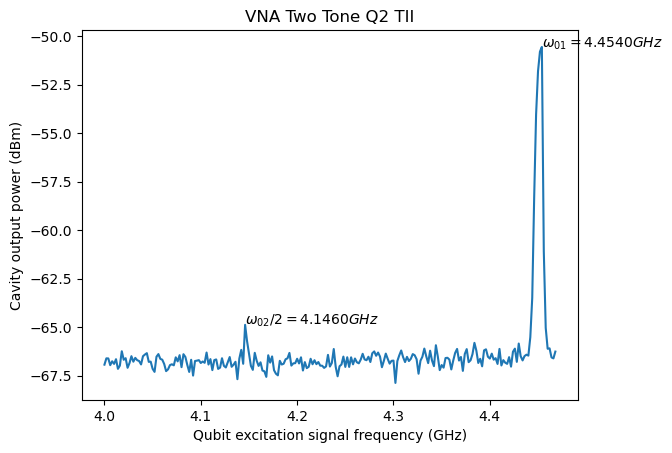
\includegraphics[width=0.5\linewidth]{images/vna-two-tone.png}
    \caption{Frequency domain scan of the qubit excitation signal with the y-axis being the output amplitude of the cavity at cavity resonance. One can notice both the excitation to the first level of the qubit in the higher peak and the 2 photon excitation from the ground to the second level in the lower peak.}
    \label{fig:TIIQ2-vna-2tone}
\end{figure}

\begin{figure}[H]
    \centering
    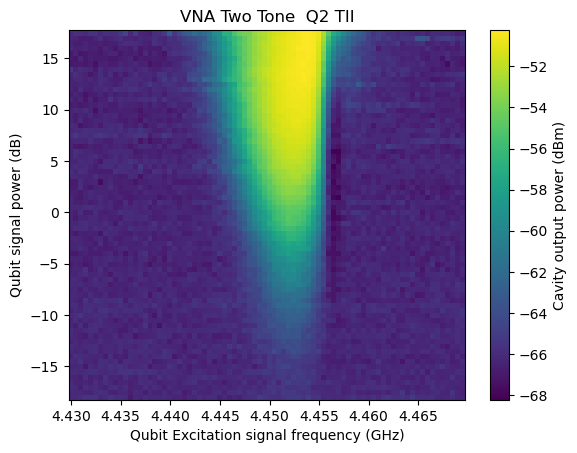
\includegraphics[width=0.5\linewidth]{images/vna-2-tone-map-1.png}
    \caption{Frequency domain and power scan of the qubit excitation signal with the color-axis being the output amplitude of the cavity at cavity resonance.}
    \label{fig:TIIQ2-vna-}
\end{figure}

\begin{figure}[H]
    \centering
    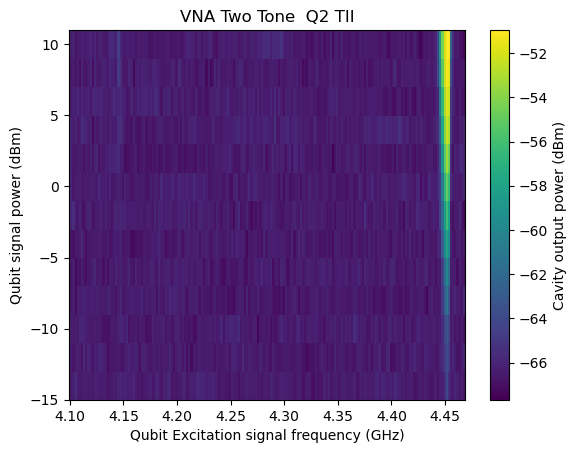
\includegraphics[width=0.5\linewidth]{images/vna-2-tone-2.png}
    \caption{Frequency domain and power scan of the qubit excitation signal with the color-axis being the output amplitude of the cavity at cavity resonance. One can notice besides the main transition the $0\arrowright 2$ as seen in figure \ref{fig:TIIQ2-vna-2tone}.}
    \label{fig:TIIQ2-vna-}
\end{figure}
\subsubsection{The pulsed setup}
In the pulsed setup we get a slightly different resonance frequency for the cavity of 7.0208GHz and for the qubit of 4.4565GHz. Those will be used for the rest of the measurements in the pulsed setup.
\begin{figure}[H]
    \centering
    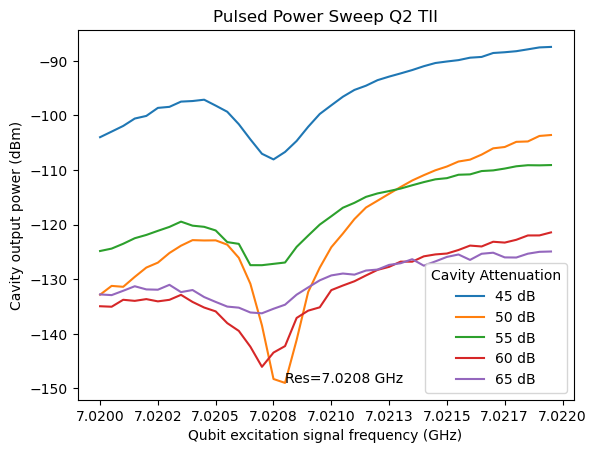
\includegraphics[width=0.5\linewidth]{images/pulsed-punchout.png}
    \caption{Frequency domain scan of the qubit excitation signal with the y-axis being the output amplitude of the cavity at cavity resonance for multiple attenuations in the cavity signal.}
    \label{fig:TIIQ2-pulsed-punchout}
\end{figure}

\begin{figure}[H]
    \centering
    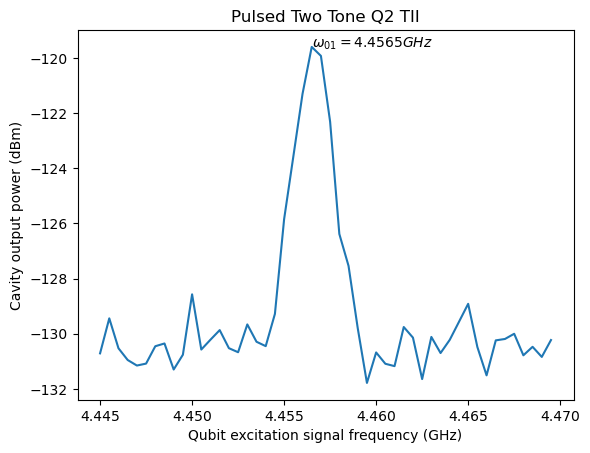
\includegraphics[width=0.5\linewidth]{images/pulsed-2-tone.png}
    \caption{Frequency domain scan of the qubit excitation signal with the y-axis being the output amplitude of the cavity at cavity resonance.}
    \label{fig:TIIQ2-pulsed-2tone}
\end{figure}
\subsubsection{The Rabi Oscillation}
With the Rabi oscillation experiment we find the length of the $\pi$ pulse to be $\pi_{pulse}= 0.720\mu s$ which we can use to do the other measurements.
\begin{figure}[H]
    \centering
    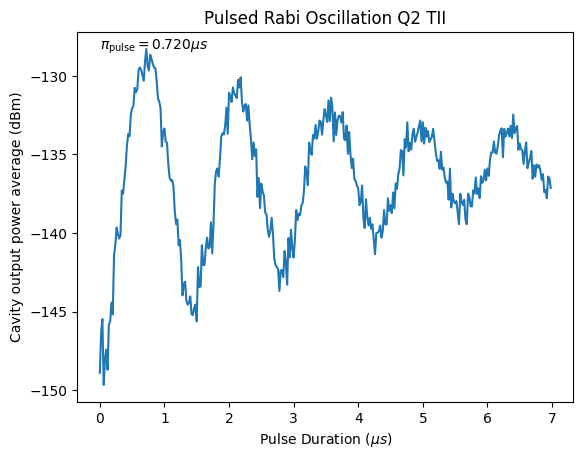
\includegraphics[width=0.5\linewidth]{images/pulsed-rabi.png}
    \caption{Rabi oscillation of the average power amplitude on the output of the cavity by changing the length of the excitation pulse of the qubit at resonant frequency.}
    \label{fig:TIIQ2-pulsed-rabi}
\end{figure}
\begin{figure}[H]
    \centering
    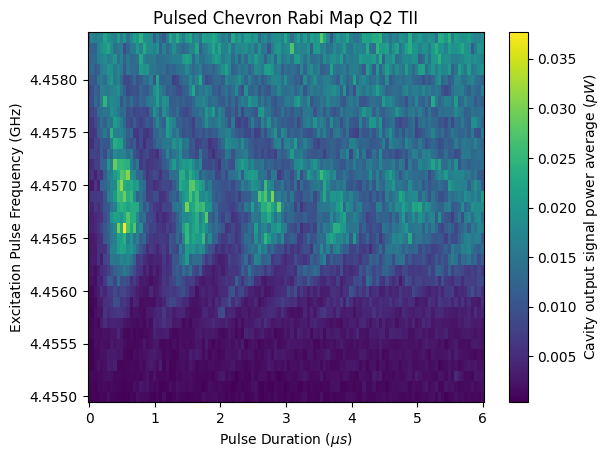
\includegraphics[width=0.5\linewidth]{images/pulsed-rabi-map.png}
    \caption{Rabi oscillation map of the average power amplitude  on the output of the cavity (color-axis) by changing the length of the excitation pulse of the qubit and the frequency corresponding to a detuning from the resonant frequency.}
    \label{fig:TIIQ2-pulsed-rabi-map}
\end{figure}

\subsubsection{The $T_1$ measurement}
\begin{figure}[H]
    \centering
    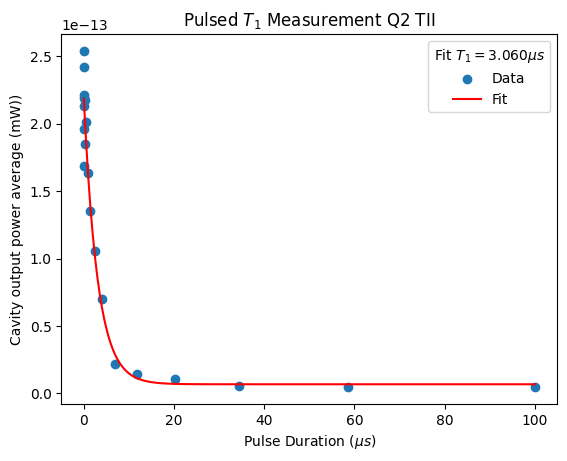
\includegraphics[width=0.5\linewidth]{images/pulsed-t1.png}
    \caption{Measurement of the $T_1$ parameter of the qubit by waiting to measure after a pi pulse}
    \label{fig:TIIQ2-pulsed-}
\end{figure}

%\subsubsection{The $T_2^*$ measurement or Ramsey Interferometry}


\subsubsection{The $T_2^{\textbf{ECHO}}$ measurement }
\begin{figure}[H]
    \centering
    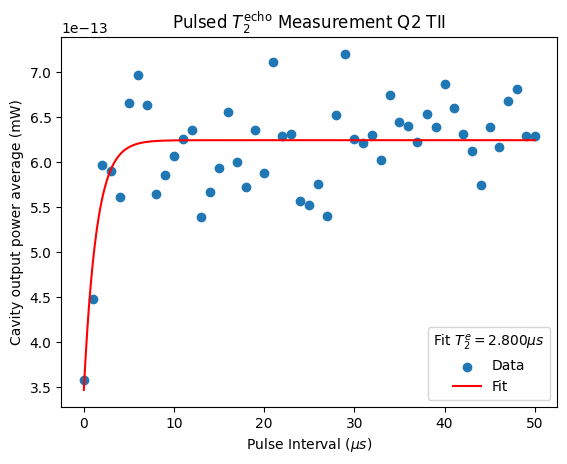
\includegraphics[width=0.5\linewidth]{images/pulsed-echo.png}
    \caption{$T_2^{echo}$ measurement made by applying a pi/2 pulse followed by a pi pulse and another pi/2 pulse with intervals of length T between them. }
    \label{fig:TIIQ2-pulsed-echo}
\end{figure}
\subsection{The 3QTII sample}
The expected parameters for this qubit calculated from the project's dimensions and parameters are 7.1GHz for the cavity resonance and 5GHz for the qubit resonance.


I skipped the VNA part by using the one made by a laboratory colleague (Ednilson) on the same sample. He got the values: $f_{cavity att=50dB}$= 7.13954 GHz,$f_{cavity att=10dB}$= 7.14235 GHz, $\omega_{01}$ = 5.257 GHz, $\omega_{02}/2$ = 4.801GHz.


\subsubsection{The pulsed setup}
In the pulsed setup we get a slightly different resonance frequency for the cavity of 7.1421 GHz and for the qubit of $\omega_{01}=5.2647GHz$. Those will be used for the rest of the measurements in the pulsed setup.

\begin{figure}[H]
    \centering
    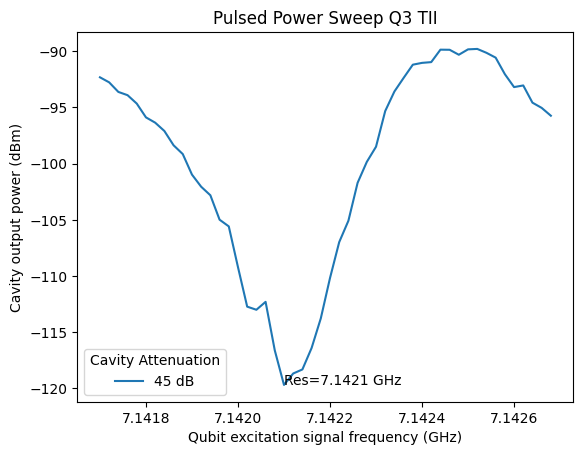
\includegraphics[width=0.5\linewidth]{images/Q3-pulsed-cavity.png}
    \caption{Frequency domain scan of the qubit excitation signal with the y-axis being the output amplitude of the cavity at cavity resonance for multiple attenuations in the cavity signal.}
    \label{fig:TIIQ3-pulsed-punchout}
\end{figure}

\begin{figure}[H]
    \centering
    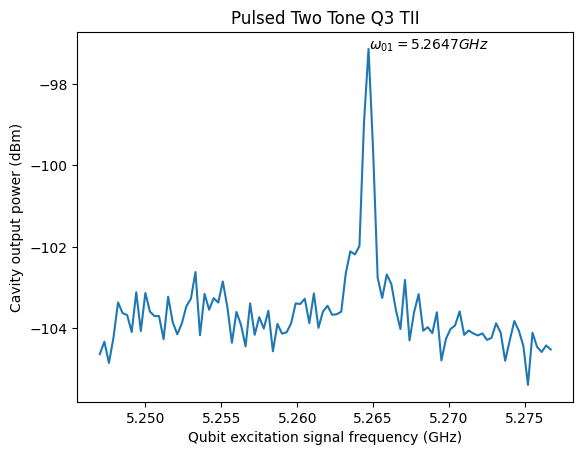
\includegraphics[width=0.5\linewidth]{images/Q3-pulsed-two-tone.png}
    \caption{Frequency domain scan of the qubit excitation signal with the y-axis being the output amplitude of the cavity at cavity resonance.}
    \label{fig:TIIQ3-pulsed-2tone}
\end{figure}

\subsubsection{The Rabi Oscillation}
With the Rabi oscillation experiment we find the length of the $\pi$ pulse to be $\pi_{\text{pulse}}=0.080\mu s$ which we can use to do the other measurements. We aim at a high power at the qubit so that we get a low Rabi period. Despite that a power that is too high can heat up the qubit stage of  the dilution refrigerator.

\begin{figure}[H]
    \centering
    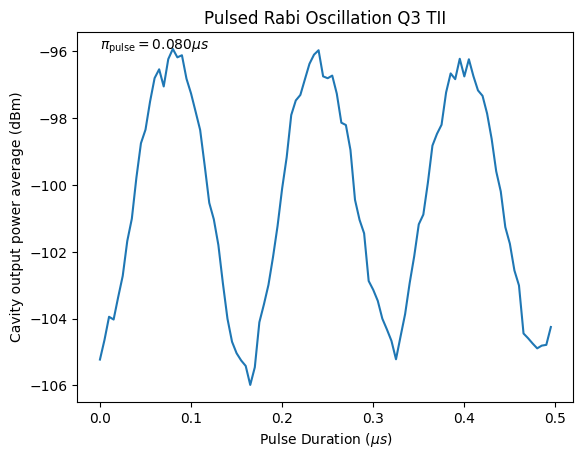
\includegraphics[width=0.5\linewidth]{images/Q3_pulsed-rabi.png}
      \caption{Rabi oscillation obtained by varying the length of the excitation pulse.}
    \label{fig:TIIQ3-pulsed-rabi}
\end{figure}
 
\subsubsection{The $T_1$ measurement}

\begin{figure}[H]
    \centering
    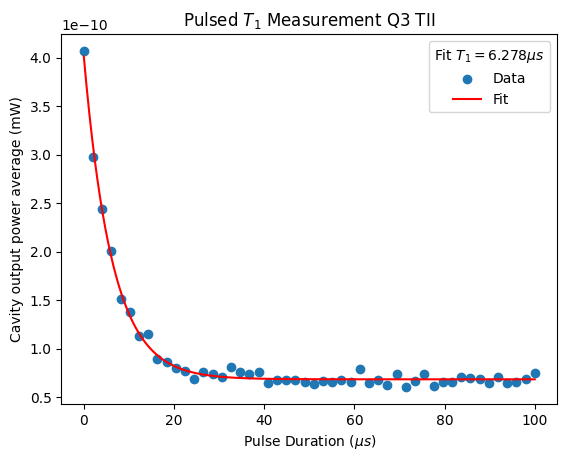
\includegraphics[width=0.5\linewidth]{images/Q3-T1.png}
    \caption{Measurement of the $T_1$ parameter of the qubit by waiting to measure after a pi pulse}
    \label{fig:TIIQ3-pulsed-T1}
\end{figure}


\subsubsection{The $T_2^*$ measurement or Ramsey Interferometry}


\begin{figure}[H]
    \centering
    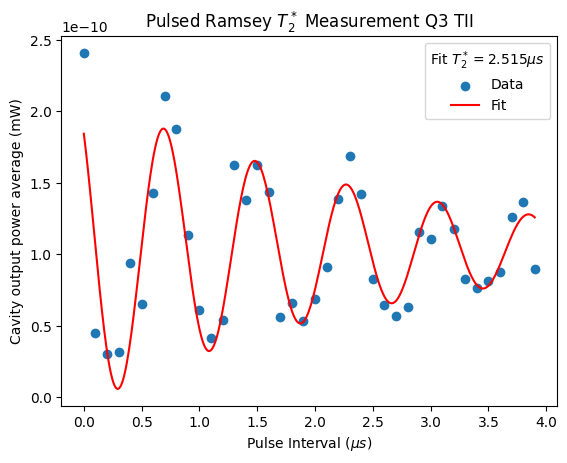
\includegraphics[width=0.5\linewidth]{images/Q3-Ramsey.png}
    \caption{$T_2^*$ measurement obtained by changing the distance between two pi/2 pulses.}
    \label{fig:TIIQ3-T2}
\end{figure}

\subsubsection{The $T_2^{\textbf{ECHO}}$ measurement }

\begin{figure}[H]
    \centering
    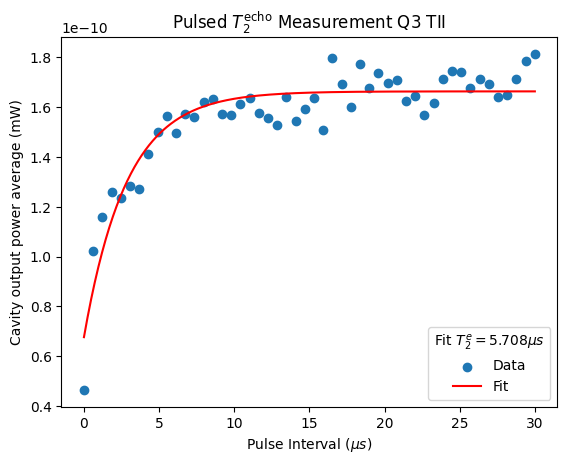
\includegraphics[width=0.5\linewidth]{images/Q3-echo.png}
    \caption{$T_2^{echo}$ measurement made by applying a pi/2 pulse followed by a pi pulse and another pi/2 pulse with pulse intervals of length T between them.  }
    \label{fig:TIIQ3-echo}
\end{figure}

Since the $T^{echo}_2$ is typically larger than the actual $T_2$ and $T^*_2$ is typically smaller we get the following approximate bounds for Q3's $T_2$  are $2.515\mu s\le T_2 \le 5.708\mu s$.

\subsubsection{The position of the cavity resonance with an excited qubit}
Here we find the position of the cavity resonance valley $f_{\textrm{cavity excited qubit}}=7.14115GHz$  from where we can calculate the coupling parameters from the the Jaynes-Cummings Hamiltonian in the dispersive approximation  $\chi=(f_{cavity}-f_{\textrm{cavity excited qubit}})/2$=0.5250MHz  and  g=$\frac{\chi}{\Delta}$=$\frac{\chi}{f_{cavity}-f_{qubit}}$=31.40MHz.

\begin{figure}[H]
    \centering
    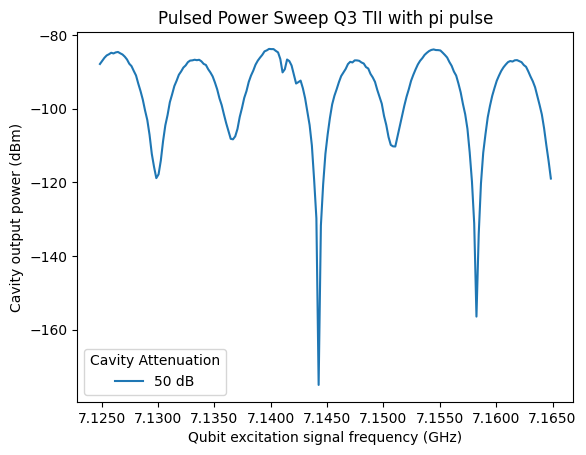
\includegraphics[width=0.5\linewidth]{images/Q3-cavity-excited.png}
    \caption{Cavity resonance valley with excited qubit with a broad range of frequencies. }
    \label{fig:cav-exc}
\end{figure}

\begin{figure}[H]
    \centering
    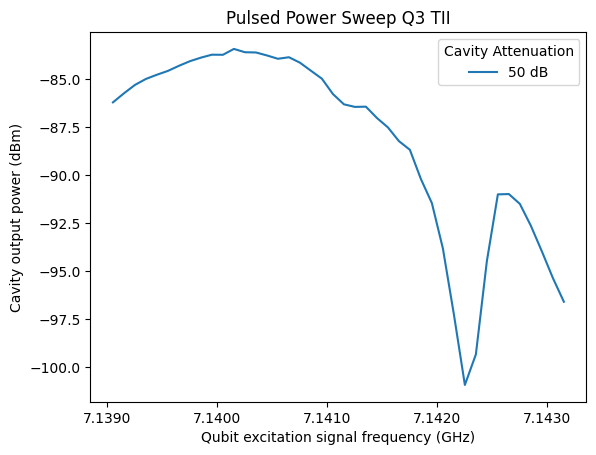
\includegraphics[width=0.5\linewidth]{images/Q3-cavity-wo-excited.png}
    \caption{Position of excited qubit cavity resonance without excitation.}
    \label{fig:cav-exc-wo}
\end{figure}

\begin{figure}[H]
    \centering
    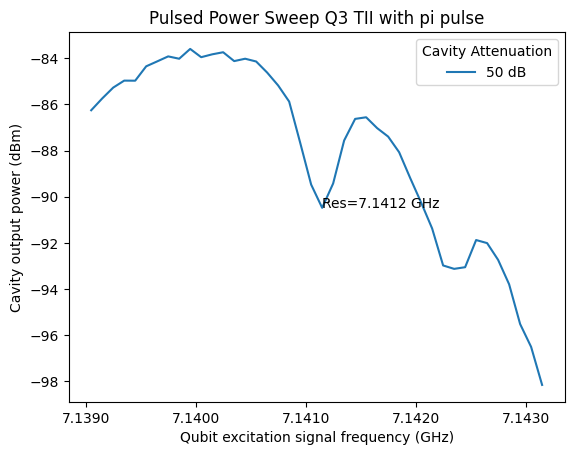
\includegraphics[width=0.5\linewidth]{images/Q3-excited-cavity-zoom.png}
    \caption{Cavity resonance valley with excited qubit. You can see that when the qubit is excited, contrary to \ref{fig:cav-exc-wo} at the same range, it appears.}
    \label{fig:cav-exc-zoom}
\end{figure}
\subsection{The 4QTII sample}
The expected parameters for this qubit calculated from the project's dimensions and parameters are 7.4GHz for the cavity resonance and 3.78GHz for the qubit resonance.

\subsubsection{The punchout}
From these measurements we get the value of the cavity resonance at low power (dressed state) of 7.443GHz that will be used to calibrate the measurement of the qubit. We also have chosen the attenuation of 50dB to be the closest to the regimen that fits best our approximations.

\begin{figure}[H]
    \centering
   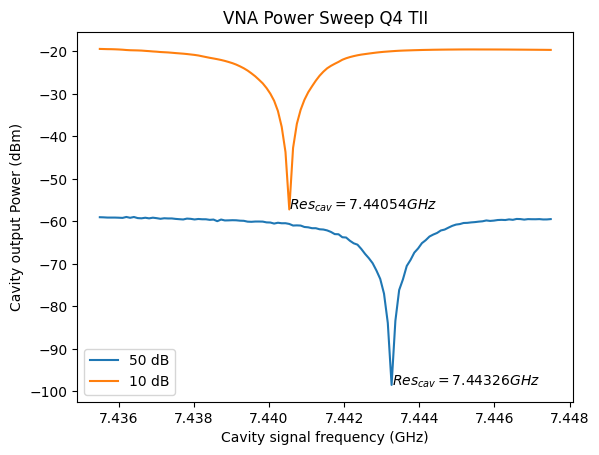
\includegraphics[width=0.5\linewidth]{images/Q4-vna-pwr-sweep.png}
    \caption{Frequency domain scan of the cavity for two different powers, with 50dB and 10 dB attenuation, and respective resonance frequencies of 7.4432GHz and 7.4405GHz. The 10dB has high power and therefore corresponds to the bare cavity  resonance frequency, the 50dB resonance corresponds to the dressed cavity.}
    \label{fig:TIIQ4-vna-punchout}
\end{figure}


\begin{figure}[H]
    \centering
       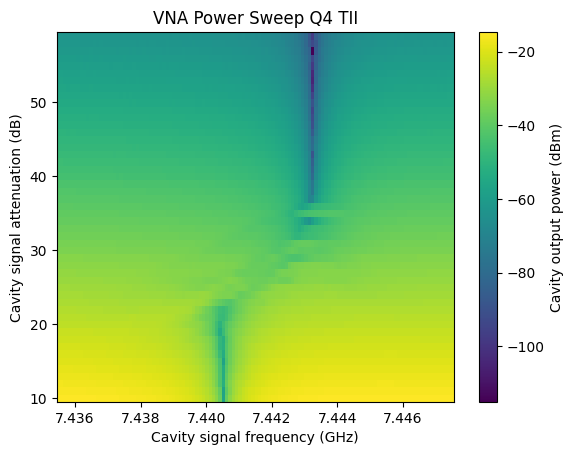
\includegraphics[width=0.5\linewidth]{images/Q4-vna-punchout-map.png}
    \caption{Frequency domain and power scan map of the cavity. The two vertical valley lines correspond to the bare and dressed cavity resonances.}
    \label{fig:TIIQ4-vna-punchout-map}
\end{figure}

\subsubsection{The Two Tone Spectroscopy}
We got from this measurement the qubit's resonance frequency for the first transition $\omega_{01}$ of 3.963GHz and for the two photon transition from the ground to the second level $\omega_{02}/2$ of 3.808GHz. Giving an aharmonicity to the qubit of $\omega_{01} -\omega_{12}=2\omega_{01} -\omega_{02}=$ 310MHz.


%\begin{figure}[H]
%    \centering
%    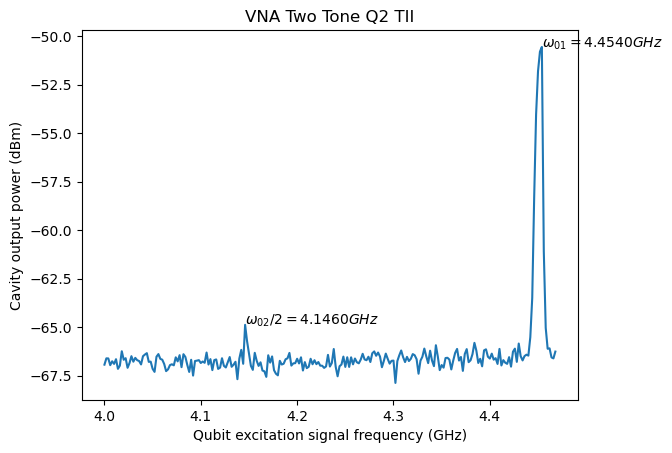
\includegraphics[width=0.5\linewidth]{images/vna-two-tone.png}
%    \caption{Frequency domain scan of the qubit excitation signal with the y-axis being the output amplitude of the cavity at cavity resonance. One can notice both the excitation to the first level of the qubit in the higher peak and the 2 photon excitation from the ground to the second level in the lower peak.}
%    \label{fig:TIIQ4-vna-2tone}
%\end{figure}

\begin{figure}[H]
    \centering
  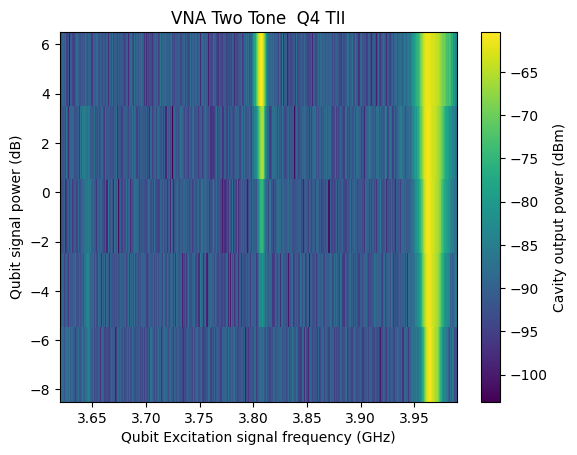
\includegraphics[width=0.5\linewidth]{images/Q4-two-tone-map.png}
    \caption{Frequency domain and power scan of the qubit excitation signal with the color-axis being the output amplitude of the cavity at cavity resonance.}
    \label{fig:TIIQ4-vna-twotonemap}
\end{figure}

\subsubsection{The pulsed setup}
In the pulsed setup we get a slightly different resonance frequency for the cavity of 7.444GHz and for the qubit of 3.9698GHz. Those will be used for the rest of the measurements in the pulsed setup.


\begin{figure}[H]
    \centering
   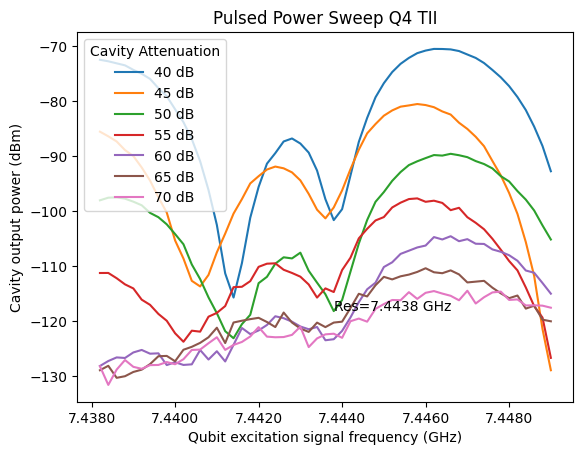
\includegraphics[width=0.5\linewidth]{images/Q4-pulsed-punchout.png}
    \caption{Frequency domain scan of the qubit excitation signal with the y-axis being the output amplitude of the cavity at cavity resonance for multiple attenuations in the cavity signal.}
    \label{fig:TIIQ4-pulsed-punchout}
\end{figure}

\begin{figure}[H]
    \centering
    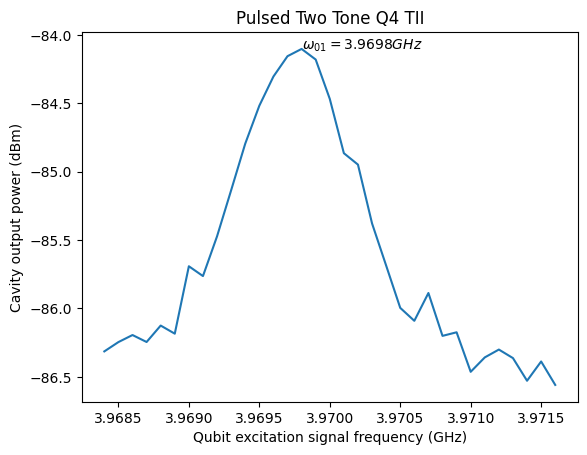
\includegraphics[width=0.5\linewidth]{images/Q4-pulsed-2-tone.png}
    \caption{Frequency domain scan of the qubit excitation signal with the y-axis being the output amplitude of the cavity at cavity resonance.}
    \label{fig:TIIQ4-pulsed-2tone}
\end{figure}

\subsubsection{The Rabi Oscillation}
With the Rabi oscillation experiment we find the length of the $\pi$ pulse to be $\pi_{pulse}= 0.700\mu s$ which we can use to do the other measurements.

\begin{figure}[H]
    \centering
     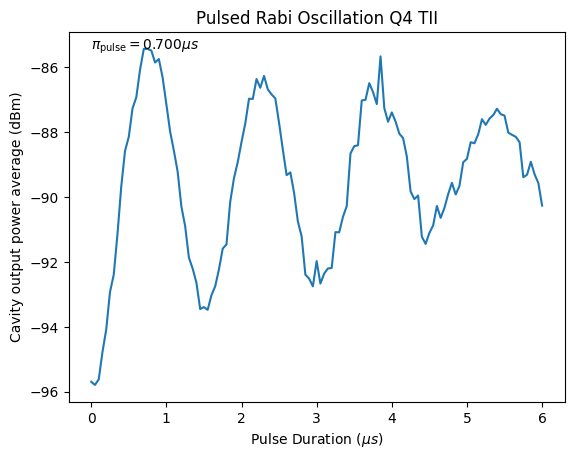
\includegraphics[width=0.5\linewidth]{images/Q4-rabi.png}
    \caption{Rabi oscillation of the average power amplitude on the output of the cavity by changing the length of the excitation pulse of the qubit at resonant frequency.}
    \label{fig:TIIQ4-pulsed-rabi}
\end{figure}

\subsubsection{The $T_1$ measurement}
\begin{figure}[H]
    \centering
       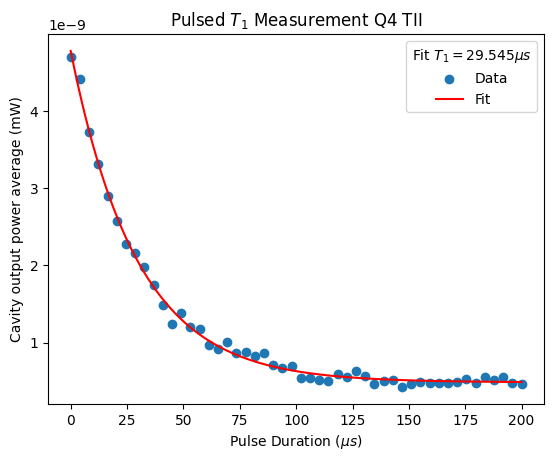
\includegraphics[width=0.5\linewidth]{images/Q4-T1.png}
    \caption{Measurement of the $T_1$ parameter of the qubit by waiting to measure after a pi pulse}
    \label{fig:TIIQ4-T1}
\end{figure}

\subsubsection{The $T_2^*$ measurement or Ramsey Interferometry}

\begin{figure}[H]
    \centering
    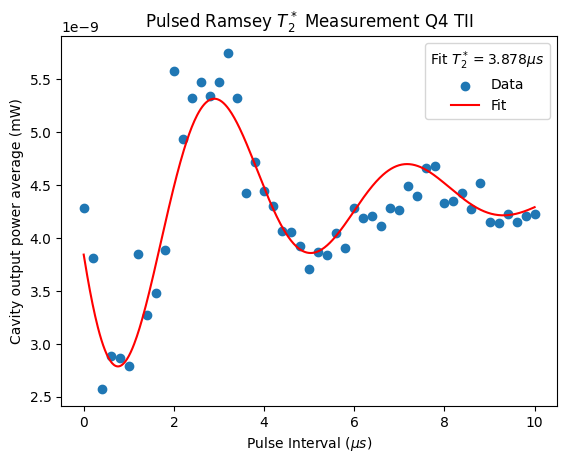
\includegraphics[width=0.5\linewidth]{images/Q4-ramsey.png}
   \caption{$T_2^*$ measurement obtained by changing the distance between two pi/2 pulses.}
    \label{fig:Q4-ramsey}
\end{figure}

\subsection{The $T_2^{\textbf{ECHO}}$ measurement }

\begin{figure}[H]
    \centering
    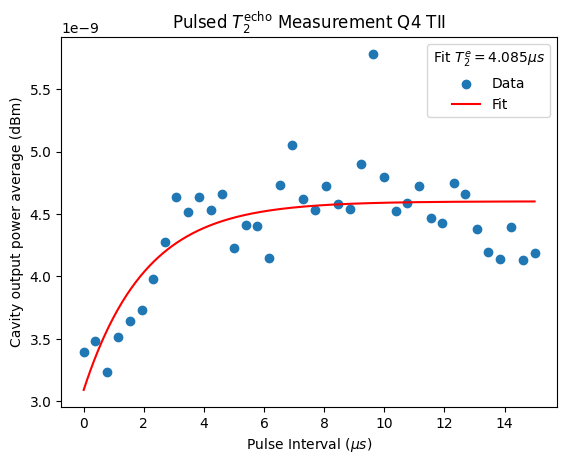
\includegraphics[width=0.5\linewidth]{images/Q4-echo.png}
    \caption{$T_2^{echo}$ measurement made by applying a pi/2 pulse followed by a pi pulse and another pi/2 pulse with intervals of length T between them.  }
    \label{fig:TIIQ4-echo}
\end{figure}

\part*{Discussion}
\emph{ To be redacted and included in the next report when the simulations are finished.}

\part*{Conclusion}
In this part of the internship, a good familiarity with the equipment and procedures was developed, as well as a proper understanding of the generated data and the proper interpretation we give it using the theories of quantum mechanics. Another point that could be learned was the limitation of the quantum mechanical model in describing real physical phenomena through the decoherence of the system and the resulting tests that enable us to evaluate this decoherence and measure it through the parameters $T_!$and $T_2$ inferred from these tests.
\printbibliography
\end{document}

